\section{Diseño del sistema}
\subsection{Del análsis al diseño}

\subsection{Diagramas UML}

\subsubsection{Diagramas de Casos de uso y estados}


\begin{figure}[h]
\begin{center}
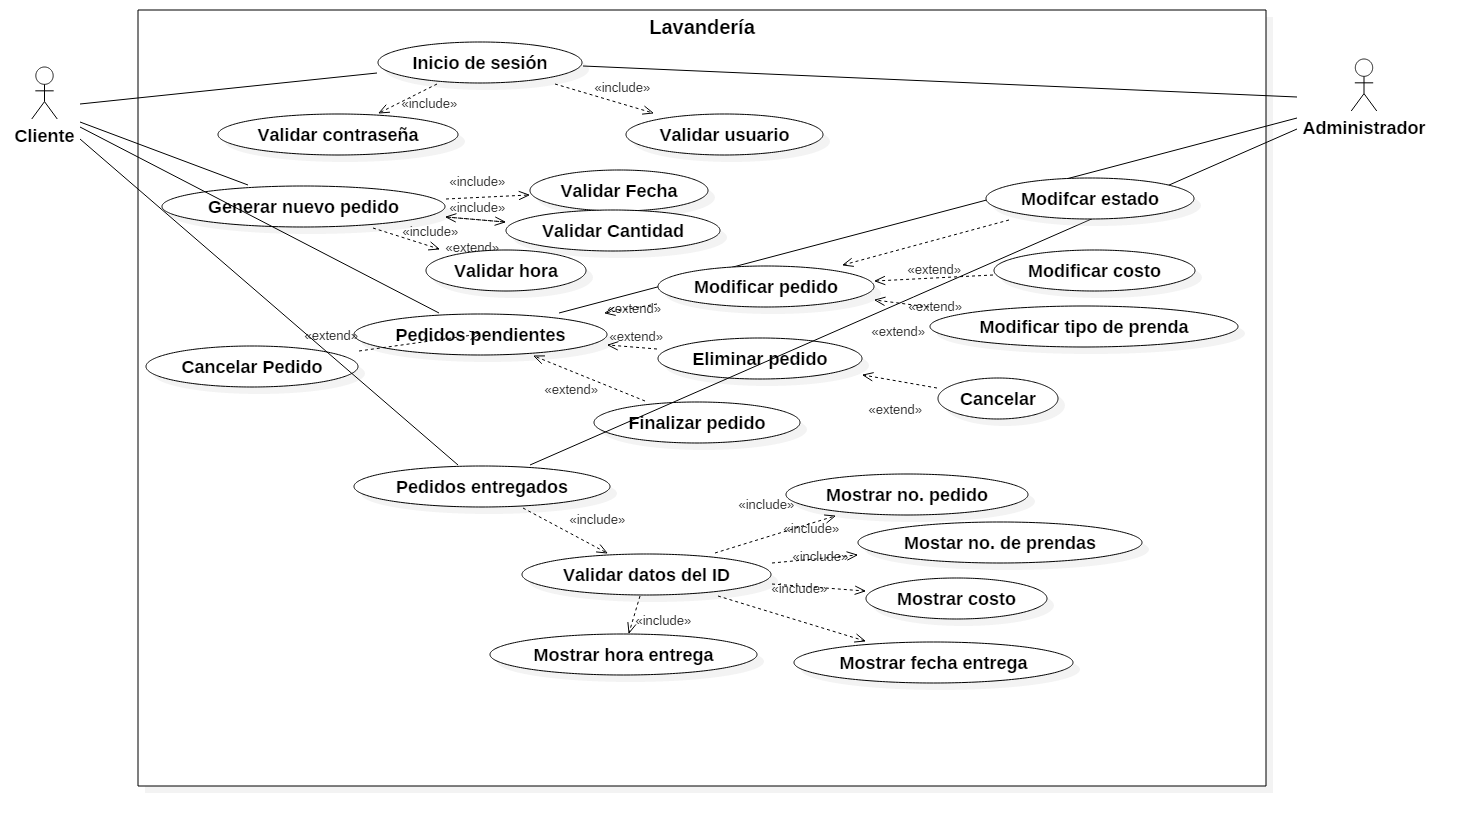
\includegraphics[width=8cm]{./imagenes/diagramas/CU_Lavanderia.png}
\end{center}
\caption{CU general del sistema}
\end{figure}


\begin{figure}[h]
\begin{center}
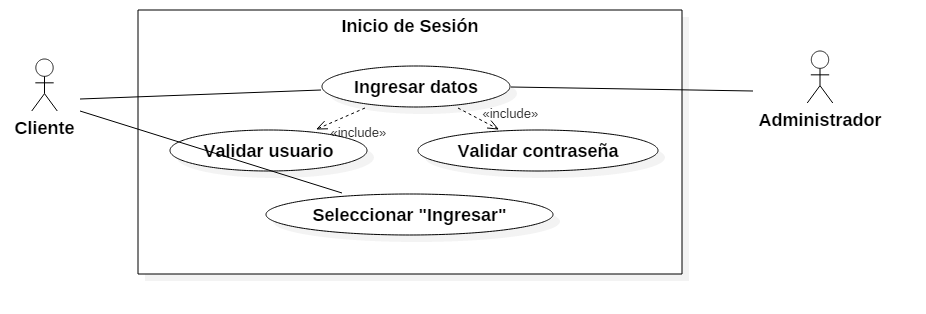
\includegraphics[width=8cm]{./imagenes/diagramas/CU_IniciarSesion.png}
\end{center}
\caption{Inicio de sesión}
\end{figure}


\begin{figure}[h]
\begin{center}
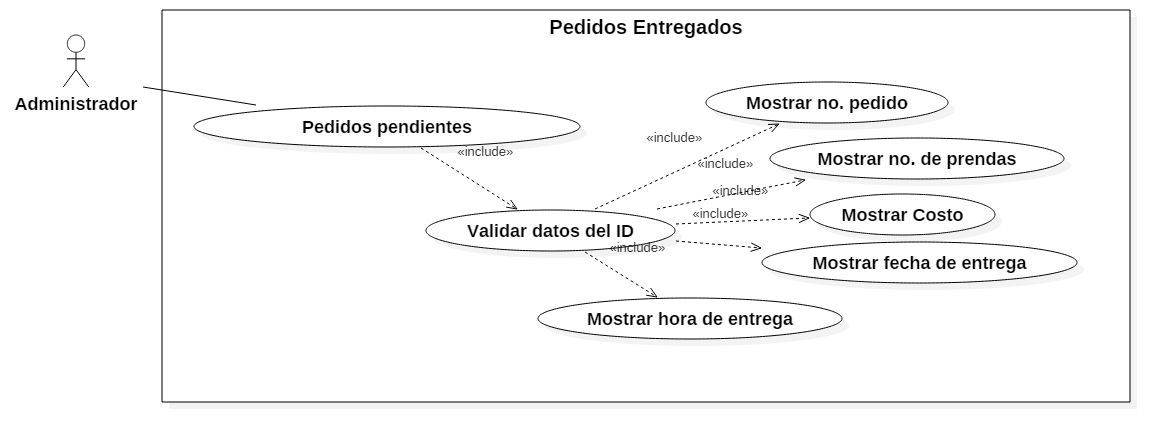
\includegraphics[width=8cm]{./imagenes/diagramas/CU_PedidosEntregados(Admin).png}
\end{center}
\caption{CU de Pedidos entregados del Administrador}
\end{figure}


\begin{figure}[h]
\begin{center}
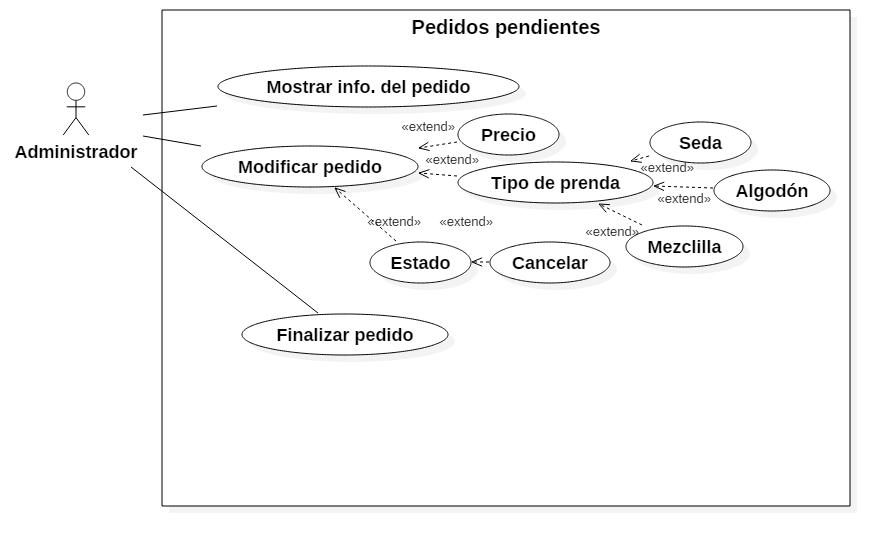
\includegraphics[width=8cm]{./imagenes/diagramas/CU_PedidosPendientes(Admin).png}
\end{center}
\caption{CU de pedidos pendientes del Administrador}
\end{figure}


\begin{figure}[h]
\begin{center}
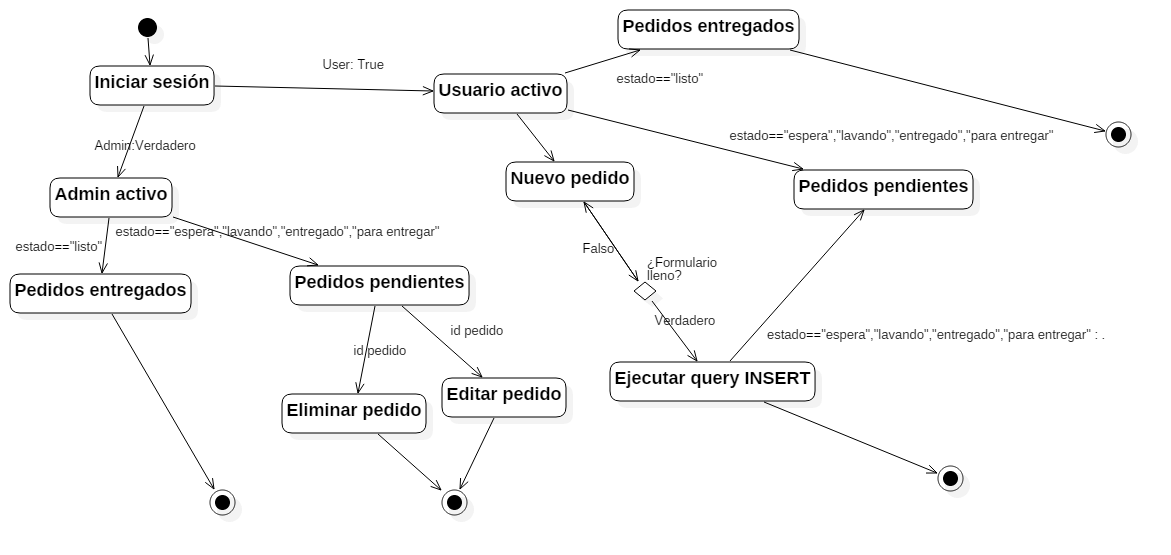
\includegraphics[width=8cm]{./imagenes/diagramas/Estado_lavanderia.png}
\end{center}
\caption{Diagrama de estados del sistema}
\end{figure}


\begin{figure}[h]
\begin{center}
\includegraphics[width=8cm]{./imagenes/diagramas/Estados_lavanderia2.png}
\end{center}
\caption{Diagrama de estados de un nuevo pedido}
\end{figure}
\newpage

\subsubsection{Diagramas de clases y objetos}




\subsubsection{Diagramas de procesos y actividades}






\subsubsection{Diagramas de secuencia y colaboracion}




\subsubsection{Diagrama de componentes y distribucion}

